\chapter{Appendices}\label{chapter:appendices}

\section{CAP Theorem}\label{section:appendices/CAP_theorem}
CAP Theorem is published by scientist Eric Brewer and also called as Brewer's Theorem. There are three major requirements for deploying an application in a distributed environment.
\begin{enumerate}
\item \textbf{Consistency}\\
A functionality of a service is accomplished as a whole or not at all. All the nodes accessing any data see the same version at any given time.
\item \textbf{Availability}\\
The functionalities provided by a service are available and working.
\item \textbf{Partition Tolerance}\\
The partitions which occurs due to problems in the network does not affect the operations of the system unless the whole network fails.
\end{enumerate}
According to the theorem, as the system scales across a number of nodes and the volume of requests increases, it becomes difficult to achieve all the three qualities but to compromise any one of them \cite{Julian:2009aa}. 
Network partitions cannot be avoided completely due to the very nature of distributed system and so is the quality of partition tolerance has to be maintained. The choice is the trade off between availability and consistency. It is completely dependent upon business requirement which one to choose. \cite{Peter-Bailis:2013aa}
\section{Eventual Consistency}\label{section:appendices/eventual_consistency}
It is a weaker form of consistency which guarantees that all read to a data item return the same value eventually, if no additional updates are performend to the same data item. For any update, only the nodes which are viable and reachable at the moment are updated and the remaining nodes are updated when they are back online. \cite{Peter-Bailis:2013aa}
\section{Command Query Responsibility Segregation(CQRS)}\label{section:appendices/CQRS}
In this pattern as shown in the figure \ref{fig:appendices/cqrs}, the conceptual model is divided into two separate models, each one for update and read. It refers to creating different object model handled by different logical processes. The database can be shared, where it acts as an integration point but can have different database as well.

\begin{figure}[H]
\begin{center}
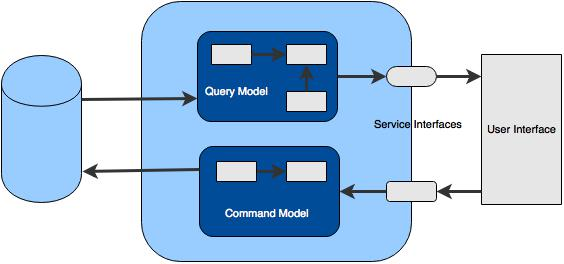
\includegraphics[width=0.8\textwidth]{figures/Appendices_one_cqrs}
\caption{CQRS [\cite{Fowler:2011ab}]}
\label{fig:appendices/cqrs}
\end{center}
\end{figure}

\section{Single Responsibility Principle}\label{section:appendices/single_responsibility_principle}
A responsibility is inferred as a reason to change. According to the principle, a service should have a single reson to change. In order to achieve that, a service should perform functionalities which change for the same reason. \cite{Martin:2009aa} \cite{Stine:2014aa}

\section{BlueGreen Deployment}\label{section:appendices/blue_green_deployment}
Continuous Delivery focus on rolling out the changes as fast as possible from development to production. However, during the process of releasing there can be subtle amount of downtime or possibility of errors. With the intention to tackle that, bluegreen deployment introduces an approach by creating two identical production environments "blue" and "green" with one active at a time "blue". At this time a routing mechanism points all traffic towards "blue" environment. Whenever any change has to be rolled out, it is done in "green" environment. As soon as the environment is fully tested, the routing mechanism points all traffic towards "green" environment. In this way, there is negligible amount of downtime and in the event of any problem, the traffic can be routed back to old "blue" environment.

\section{Canary Release}\label{section:appendices/canary_release}
Canary Relase is an approach to minimize the risk of releasing faulty application to all users. Similar to the bluegreen deployment, there are two identical production environments. As one environment is serving live requests, another environment is used to deploy new changes. After the changes are tested properly, the routing mechanism exposes few selected users to the new environment to minimize the risk. As the new system gains confidence, it is rolled out to large group of users and ultimately to all users.